\begin{figure*}[t]
\centering
\begin{subfigure}[b]{0.49\textwidth}
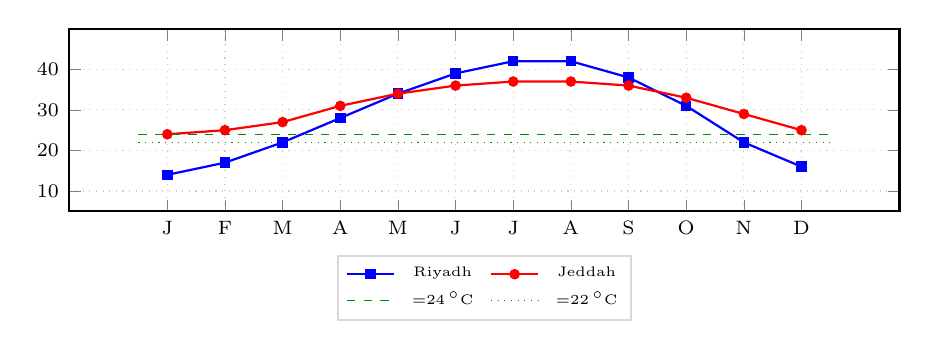
\begin{tikzpicture}
\begin{axis}[
  width=\linewidth, height=3.9cm,
  xtick={1,...,12},
  xticklabels={J,F,M,A,M,J,J,A,S,O,N,D},
  xticklabel style={font=\scriptsize},
  ymin=5, ymax=50, ytick={10,20,30,40},
  grid=major,grid style={dotted,gray!40},
  legend style={at={(0.5,-0.24)},anchor=north,
                legend columns=2,font=\tiny,
                draw=gray!30,column sep=4pt},
  tick label style={font=\scriptsize},
  label style={font=\small},thick
]
\addplot[blue,thick,mark=square*,mark size=1.5pt]
  coordinates{(1,14)(2,17)(3,22)(4,28)(5,34)(6,39)
              (7,42)(8,42)(9,38)(10,31)(11,22)(12,16)};
\addlegendentry{Riyadh}
\addplot[red,thick,mark=*,mark size=1.5pt]
  coordinates{(1,24)(2,25)(3,27)(4,31)(5,34)(6,36)
              (7,37)(8,37)(9,36)(10,33)(11,29)(12,25)};
\addlegendentry{Jeddah}
\addplot[green!55!black,dashed,thin]
  coordinates{(0.5,24)(12.5,24)};
\addlegendentry{$\Tmax{=}24\,^\circ$C}
\addplot[green!55!black,dotted,thin]
  coordinates{(0.5,22)(12.5,22)};
\addlegendentry{$\Tmin{=}22\,^\circ$C}
\end{axis}
\end{tikzpicture}
\caption{Monthly mean temperatures.}
\end{subfigure}\hfill
\begin{subfigure}[b]{0.49\textwidth}
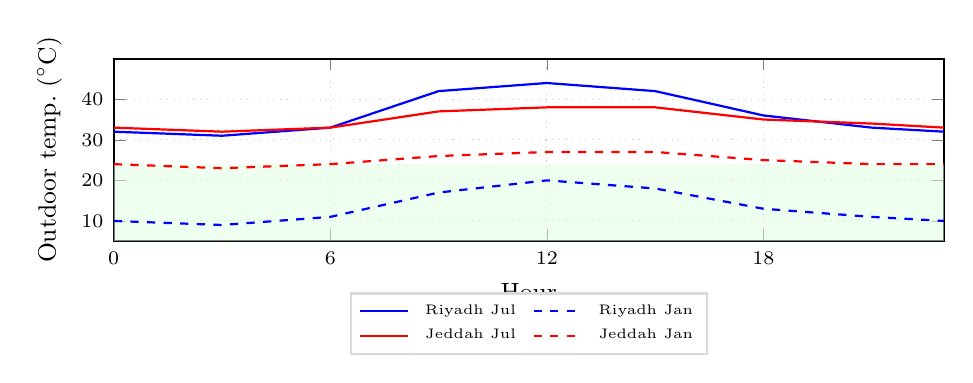
\begin{tikzpicture}
\begin{axis}[
  width=\linewidth, height=3.9cm,
  xlabel={Hour}, ylabel={Outdoor temp.\ ($^\circ$C)},
  xmin=0,xmax=23, xtick={0,6,12,18},
  ymin=5, ymax=50, ytick={10,20,30,40},
  grid=major,grid style={dotted,gray!40},
  legend style={at={(0.5,-0.28)},anchor=north,
                legend columns=2,font=\tiny,
                draw=gray!30,column sep=4pt},
  tick label style={font=\scriptsize},
  label style={font=\small},thick
]
\addplot[fill=green!12,draw=none,opacity=0.5,forget plot]
  coordinates{(0,22)(0,24)(23,24)(23,22)}\closedcycle;
\addplot[blue,thick]
  coordinates{(0,32)(3,31)(6,33)(9,42)(12,44)(15,42)(18,36)(21,33)(23,32)};
\addlegendentry{Riyadh Jul}
\addplot[blue,thick,dashed]
  coordinates{(0,10)(3,9)(6,11)(9,17)(12,20)(15,18)(18,13)(21,11)(23,10)};
\addlegendentry{Riyadh Jan}
\addplot[red,thick]
  coordinates{(0,33)(3,32)(6,33)(9,37)(12,38)(15,38)(18,35)(21,34)(23,33)};
\addlegendentry{Jeddah Jul}
\addplot[red,thick,dashed]
  coordinates{(0,24)(3,23)(6,24)(9,26)(12,27)(15,27)(18,25)(21,24)(23,24)};
\addlegendentry{Jeddah Jan}
\end{axis}
\end{tikzpicture}
\caption{Hourly diurnal profiles.}
\end{subfigure}
\caption{EPW climate data. (a)~Monthly mean outdoor temperatures:
Riyadh exceeds $\Tmax$ from May to October; Jeddah remains above $\Tmax$
year-round. (b)~Hourly profiles for summer and winter: Riyadh's
$12.7\,$K cooling-season diurnal swing enables pre-cooling; Jeddah's compressed
$8.4\,$K swing demands near-continuous operation. Green shading in
(b) marks the comfort band.}
\label{fig:climate}
\end{figure*}
